\section{Microkernel and Plugin System}
\label{sec:microkernel}

GAWorld v2 combines a connected cognition pipeline with a small kernel, a
registry of fourteen built-in plugins, and compatibility-preserving domain
paths.  The K1--K5 migration audited in v1 is now closed for the defined
scope, and a v2 audit covers three further migrations: \emph{multi-tenant
world resolution} (K6), \emph{distributed hub-and-node execution} (K7), and
\emph{parallel-worlds counterfactual execution} (K8).  The
\Cref{fig:system-architecture} freezes the v2 architecture at the audited
commit; existing capability cases are predate or postdate specific migrations
and are labeled accordingly in \cref{sec:capability-cases}.

\begin{figure}[t]
  \centering
  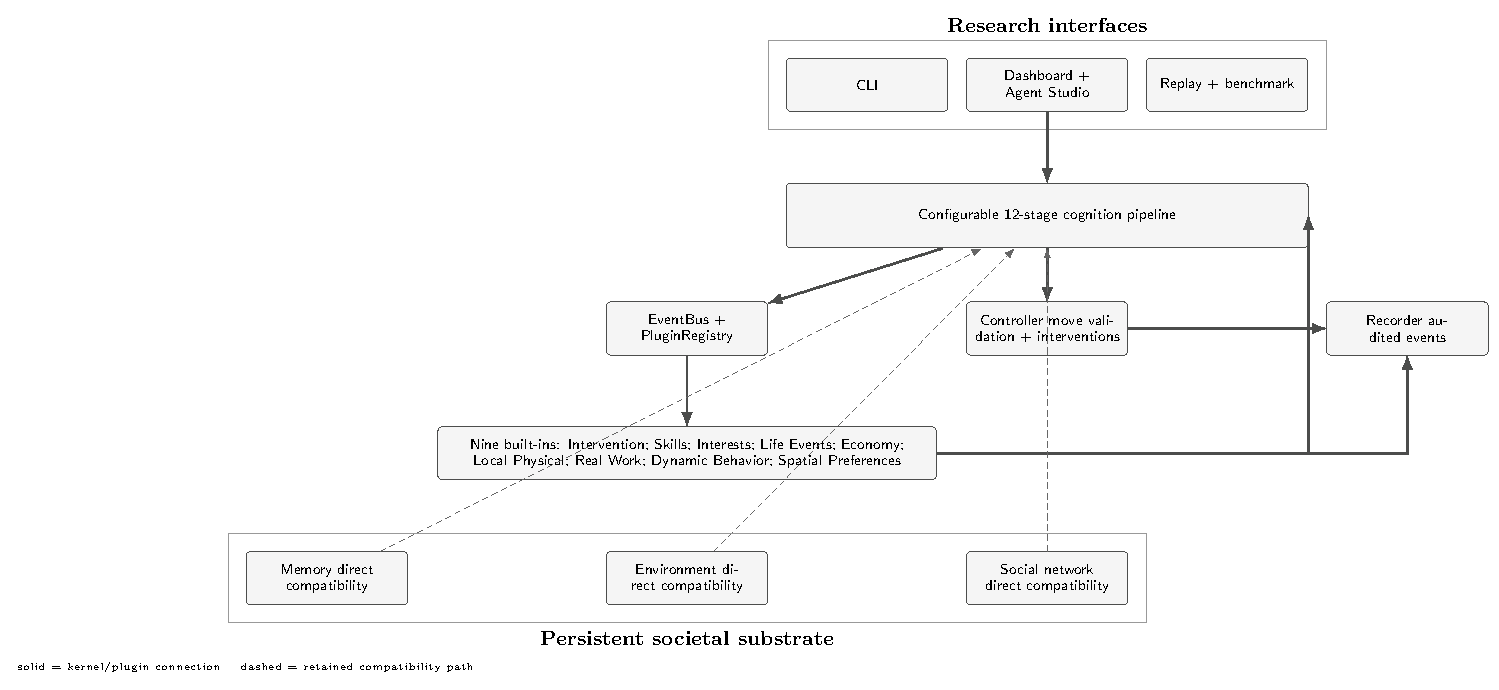
\includegraphics[width=\linewidth]{system_architecture.pdf}
  \caption{Audited v2 execution architecture.  The kernel (Clock, EventBus,
  PluginRegistry, Controller, Recorder, SimContext) serves the cognition
  pipeline and the per-tenant world resolver.  Fourteen built-ins contribute
  through the registry, bus, pipeline filters, or lifecycle events.
  Movement uses the Controller validation gate; Recorder events coexist with
  established domain-specific outputs.  In a multi-tenant deployment, the
  world resolver is the request-time entry point; in a multi-node deployment,
  the hub routes player interventions to the owning node.}
  \label{fig:system-architecture}
\end{figure}

\begin{figure}[t]
  \centering
  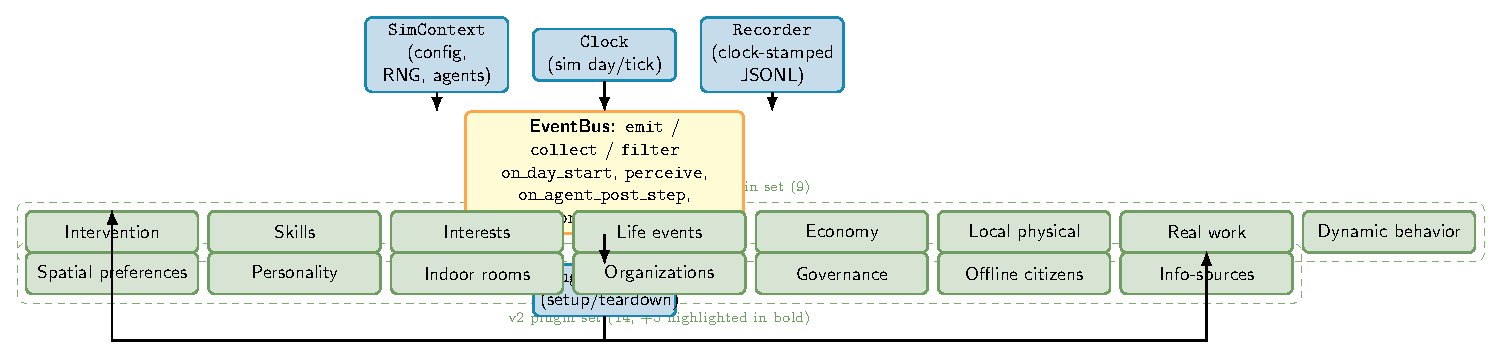
\includegraphics[width=\linewidth]{plugin_assembly.pdf}
  \caption{The fourteen v2 built-in plugins and their relationship to the
  kernel.  Plugins may subscribe to lifecycle events, contribute to
  perception, filter a value, or own namespaced state.  The v1 plugin set
  (nine) is shown above the v2 additions (five) for comparison.}
  \label{fig:plugin-assembly}
\end{figure}

\subsection{Kernel services}

\paragraph{Simulation context and clock.}
\texttt{SimContext} holds configuration, Clock, EventBus, PluginRegistry,
Controller, Recorder, agents and their identifier index, an LLM callable, a
seeded random-number generator, an \texttt{extras} compatibility escape
hatch, and (v2) a \texttt{WorldContext} reference to the active per-tenant
world.  It also provides simulation-level and per-agent plugin-state
namespaces.  The outer loop is the sole clock writer, giving stages, plugins,
and records a common simulated day, time, and tick.  This ordering does not
by itself make model calls, external services, or concurrency deterministic.

\paragraph{Event bus and plugin registry.}
The EventBus supports priority-ordered observation (\texttt{emit}), merged
contribution (\texttt{collect}), and value rewriting (\texttt{filter}).
Handler failures are logged and isolated by default, so warnings and active
plugin lists must accompany results.  The PluginRegistry assembles built-ins,
configuration-named classes, and installed entry points; orders setup by
declared dependencies; skips failed or unsatisfied plugins; and tears active
plugins down in reverse order.  Plugins may own configuration, namespaced
agent state, and output directories, but execute in process and are not a
sandbox.

\paragraph{Controller.}
The Controller provides a priority-ordered validator chain over structured
\texttt{ActionRequest}s and a named runtime-intervention API.  In the main
simulator, movement requests pass through validation: denial preserves the
origin and is surfaced in the next perception, while a rewrite can change the
destination.  The standard runtime interventions set one agent-state value,
update a dotted live-config path, queue agent removal for the next day
boundary, and (v2) deliver a player intervention to a specific node's queue.
Denials and interventions are audited through the Recorder.

\paragraph{Recorder.}
The Recorder appends clock-stamped JSON objects to table-specific files and
is closed when the simulation exits.  It records Controller activity,
distributed-hub activity, player interventions, and is available to plugins.
Main traces, state history, memories, environment events, and specialized
metrics also retain established writers.

\paragraph{World resolver (K6).}
The world resolver turns a request's authenticated user, a cookie indicating
the current world, and the caller's role into a \texttt{WorldContext} that
selects the active per-tenant configuration overlay, output root, run state,
and intervention queue.  Path-resolving functions in the dashboard and
simulation code consult the active world; module constants remain valid for
the \texttt{default} world so that single-tenant deployments and unit tests
behave identically.  When the account store is absent, the resolver
short-circuits to the \texttt{default} world.

\paragraph{Distributed hub (K7).}
The hub owns the per-world relay, the per-node intervention outbox, the
node-token store, and the global Recorder merge point.  The hub is the
\emph{dashboard server} when accounts are enabled and a thin
\texttt{cluster/hub} when accounts are not.  The hub does not advance
simulation time; it serves the run's record and routes messages.

\paragraph{Parallel-worlds engine (K8).}
The parallel-worlds engine runs up to eight matched worlds under a shared
seed and a per-world config patch, isolates each world's output tree, and
collects per-arm completion status and per-resident trajectory diffs for
post-hoc counterfactual inference.  It reuses the same event-bus,
Controller, and Recorder path; no domain code is changed between worlds.

\subsection{Built-in plugin assembly}

The audited registry assembles fourteen built-in plugins.  They attach
domain behavior to day/tick events, perception contributions, location
filters, action or outcome filters, and post-step or day-end hooks.  The
following table summarizes their declared surface and an indicative
per-agent or per-world state fragment.

\begin{table}[t]
\centering
\small
\setlength{\tabcolsep}{4pt}
\caption{The audited v2 plugin set.  Per-agent state column lists the
declarative fragment a researcher can read on a hashed run; the deployment
column lists the post-v1 changes each plugin enables.}
\label{tab:plugins}
\begin{tabular}{@{}p{0.20\linewidth}p{0.20\linewidth}p{0.18\linewidth}p{0.32\linewidth}@{}}
\toprule
Plugin & Lifecycle hook & Per-agent state fragment & v2 addition \\
\midrule
Intervention & on\_day\_start, post\_step & \texttt{ext.intervention} & cross-tenant metrics \\
Skills        & on\_agent\_post\_step, memorize & private skill library & skill consolidation by personality \\
Interests     & on\_day\_end, perceive & \texttt{ext.interests} & growth phase tracker \\
Life events   & on\_day\_start, on\_agent\_post\_step & \texttt{ext.life} & state effect normalization \\
Economy       & on\_day\_end, on\_agent\_post\_step & \texttt{state.econ} & endogenous inflation, credit-bound consumption \\
Local physical perception & perceive & local snapshot & indoor-room resolution \\
Real work     & on\_day\_start, on\_agent\_post\_step & \texttt{ext.work} & capability profile cache \\
Dynamic behavior & perceive, interrupts & \texttt{ext.dynamic} & personality-conditional interruption probability \\
Spatial preferences & filter (location) & \texttt{ext.spatial} & aversive-route rewrite \\
Personality   & agents.built, perceive & \texttt{personality} & Big-Five anchors + LLM overlay \\
Indoor rooms and venue capacity & agent.moved, perceive & \texttt{locations.room\_intent} & room-resolved occupancy and capacity \\
Organizations & on\_day\_start, on\_day\_end, on\_agent\_post\_step & \texttt{ext.org} & persistent org with role \\
Governance    & on\_day\_end, on\_day\_start & \texttt{ext.gov} & proposal/ballot engine \\
Offline citizens & agents.built & \texttt{ext.offline} & ghost taxonomy with visit / duty channel \\
\bottomrule
\end{tabular}
\end{table}

The adapters delegate calculations and specialized persistence to established
modules: migration changes orchestration and ownership, not the scientific
validity of the mechanisms.  The audit table in
\Cref{tab:migration-state} lists which subsystems have been fully
plugin-owned, which are partially integrated, and which retain direct
compatibility paths.

\subsection{Plugin authoring}
\label{sec:plugin-authoring}

A third-party plugin is a subclass of \texttt{gaworld.kernel.Plugin} with a
declared \texttt{id}, a tuple of plugin \texttt{requires} dependencies, a
\texttt{setup} method that receives \texttt{SimContext} and registers
\texttt{ctx.bus.on(...)} handlers, and a \texttt{teardown} method.  A plugin
can be installed by configuration, by entry point, or by code registration
\citep{gaworldplugin}.  Configuration and entry-point installation are
non-overlapping: a configured plugin runs even if it is not published as an
entry point.  Plugin setup failures are isolated: they produce a warning and
the affected plugin is deactivated, but the rest of the registry continues to
run.  This is intentional and is the reason the plugin set can be
reconfigured at runtime without an entire-process restart; it is also the
reason that an active plugin list, with its warnings, is part of every
research artifact.

\subsection{Migration-state audit}

\begin{table}[t]
\centering
\small
\setlength{\tabcolsep}{4pt}
\caption{Implementation state in the audited v2 repository.  ``Wired''
denotes a subsystem whose boundary is now the plugin surface; ``partial''
denotes an adapter that contributes but retains direct calls; ``retained
compatibility'' denotes a subsystem whose boundary is still the legacy
direct call.  K1--K5 cover the v1 migration; K6--K8 cover v2.}
\label{tab:migration-state}
\begin{tabular}{@{}p{0.20\linewidth}p{0.20\linewidth}p{0.18\linewidth}p{0.32\linewidth}@{}}
\toprule
Surface & Current boundary & Status (K) & Retained path and consequence \\
\midrule
Cognition & Configured 12-stage pipeline & Wired (K1) & Shared step dictionary; order and omissions must be reported \\
Extensions & EventBus and PluginRegistry & Wired (K1) & Failures may degrade rather than terminate a run \\
14 domain adapters & Policy, skills, interests, events, economy, physical, work, behavior, spatial, personality, rooms, organizations, governance, offline & Plugin-integrated (K1, K2) & Established stores and writers remain; activation needs config/plugin provenance \\
Memory & Recall, storage, consolidation, decay & Direct compatibility path (K3) & Persistent context is inspectable, not psychologically validated \\
Environment and social network & World evolution and network modules & Direct compatibility path (K3) & The full world and network models are not isolated plugins \\
Controller & Move validation, named interventions, player interventions & Connected, scoped (K4) & Other actions retain established paths; no universal-gate claim \\
Recorder & Clocked structured event writer & Connected, non-exclusive (K4) & Multiple writers remain; no single-log replay claim \\
World resolution & Cookie + account + role $\rightarrow$ WorldContext & Wired (K6) & When accounts are absent, single-tenant behaviour is preserved \\
Distributed hub & Per-world relay and per-node outbox & Wired (K7) & Best-effort delivery; no consensus, no clock synchronization \\
Parallel worlds & Up to 8 matched worlds, shared seed & Wired (K8) & Deterministic; no domain change between arms \\
\bottomrule
\end{tabular}
\end{table}

\subsection{Failure and reproducibility boundaries}

A cognition-stage exception propagates because the stage is control flow.
Bus-handler and plugin-setup failures instead warn and normally leave the
remaining run active; missing dependencies deactivate the affected plugin.
Operational resilience therefore makes a completed process different from a
complete treatment.  A reproducible artifact must include resolved stage
order, active plugin identifiers, warnings, configuration, source snapshot,
model/provider conditions, specialized outputs, the world identifier, the
node identifier (if any), and the player intervention trail (if any).  The
v1 description of K1--K5 remains accurate; v2 adds the requirement that the
artifact also record the world identifier, the node identifier, and the
per-arm completion status of every parallel-worlds study.  These additions
are not yet enforced by the kernel; the artifact ledger remains the
researcher's responsibility, with the schema documented in
\Cref{sec:validation-boundaries}.
